\documentclass{article}

\usepackage{amsfonts}
\usepackage{graphicx}
\usepackage{amssymb}
\usepackage{amsmath}
\usepackage{listings}
\usepackage{hyperref}


\DeclareMathOperator{\sech}{sech}
\newcommand{\NN}{\mathbb{N}}
\newcommand{\RR}{\mathbb{R}}
\newcommand{\QQ}{\mathbb{Q}}
\newcommand{\ZZ}{\mathbb{Z}}
\newcommand{\dV}{\;\mathrm{d}V}
\newcommand{\dA}{\;\mathrm{d}A}
\newcommand{\dx}{\;\mathrm{d}x}
\newcommand{\dy}{\;\mathrm{d}y}
\newcommand{\dz}{\;\mathrm{d}z}
\newcommand{\cA}{\mathcal{A}}
\newcommand{\Bb}{\mathcal{B}}
\newcommand{\Ww}{\mathcal{W}}
\newcommand{\Dd}{\mathcal{D}}
\newcommand{\Ss}{\mathcal{S}}
\newcommand{\Ee}{\mathcal{E}}
\DeclareMathOperator{\im}{im}

\tolerance=1
\emergencystretch=\maxdimen
\hyphenpenalty=10000
\hbadness=10000

\setlength\parindent{18pt}

\begin{document}

\Large{Lincoln Sand}


\textbf{L1.}

\textbf{318.9}:

Solve the following in three variables due to Abu Kamil:
\[x < y < z\]
\[x^2 + y^2 = z^2\]
\[xz = y^2\]
\[xy = 10\]
(Begin by setting $y = \frac{10}{x}$, $z = \frac{100}{x^3}$, and
substituting in the first equation.)


If we substitute the two hinted equalities into $x^2 + y^2 = z^2$, we get:
\[x^2 + \left(\frac{10}{x}\right)^2 = \left(\frac{100}{x^3}\right)^2\]
Solving for $x$ yields:
\[x = 2^{1/4} \sqrt{5} (-1 + \sqrt{5})^{1/4}\]

Rewriting the hinted equations and substituting into $xz = y^2$ for $y$ instead of $x$ yields a value of
\[y = \frac{2^{3/4} \sqrt{5}}{(-1 + \sqrt{5})^{1/4}}\]

Using back substitution, we finally get:
\[z = \frac{2 \cdot 2^{1/4} \sqrt{5}}{(-1 + \sqrt{5})^{3/4}}\]

If we plug these values into the four initial equations, we find that it satisfies all of them.


\textbf{318.16}:

Show that one can solve $x^3 + d = cx$ by intersecting the hyperbola
$y^2 - x^2 + \frac{d}{c} x = 0$ with the parabola $x^2 = \sqrt{c} y$.
Sketch the two conics. Find sets of values for $c$ and $d$ for which
these conics do not intersect, intersect once, and intersect twice.

From $y^2 - x^2 + \frac{d}{c} x = 0$, we get $y^2 = x^2 - \frac{d}{c} x$.

From $x^2 = \sqrt{c} y$, we get $y = \frac{x^2}{\sqrt{c}}$.

We now set $x^2 - \frac{d}{c} x = \frac{x^4}{c}$ and solve for $x$.
This gives us the solutions of $x^3 + d = cx$ through simple algebraic manipulation.

Simple algebraic manipulation:
\[x^2 - \frac{d}{c} x = \frac{x^4}{c} \implies c x^2 - d x = x^4 \implies c x - d =  x^3 \implies x^3 + d = cx\]


We equate $x^2 - \frac{d}{c} x$ from the hyperbola to $\frac{x^4}{c}$ from the parabola.

We end up with $x^4 - c x^2 + dx = 0$. The number of intersections depends
on the discriminant when calculating the roots. If the discriminant is non-real,
there is no intersection. If it's $0$, some of the roots are repeated and thus
we get one intersection. If the discriminant is non-zero and real, there
are two intersections.

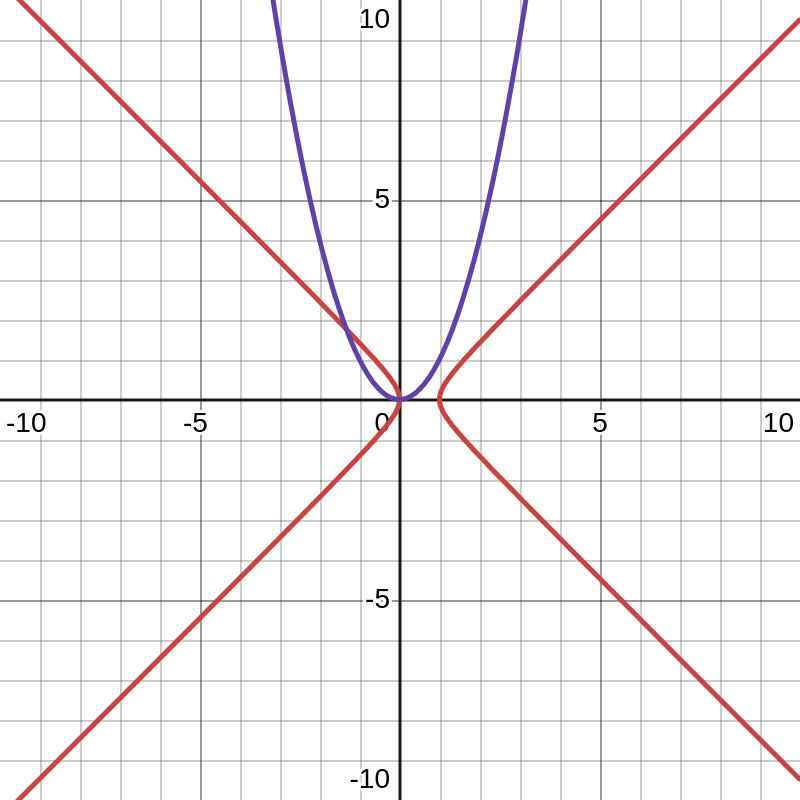
\includegraphics[width=\linewidth]{conic_pic_1.png}

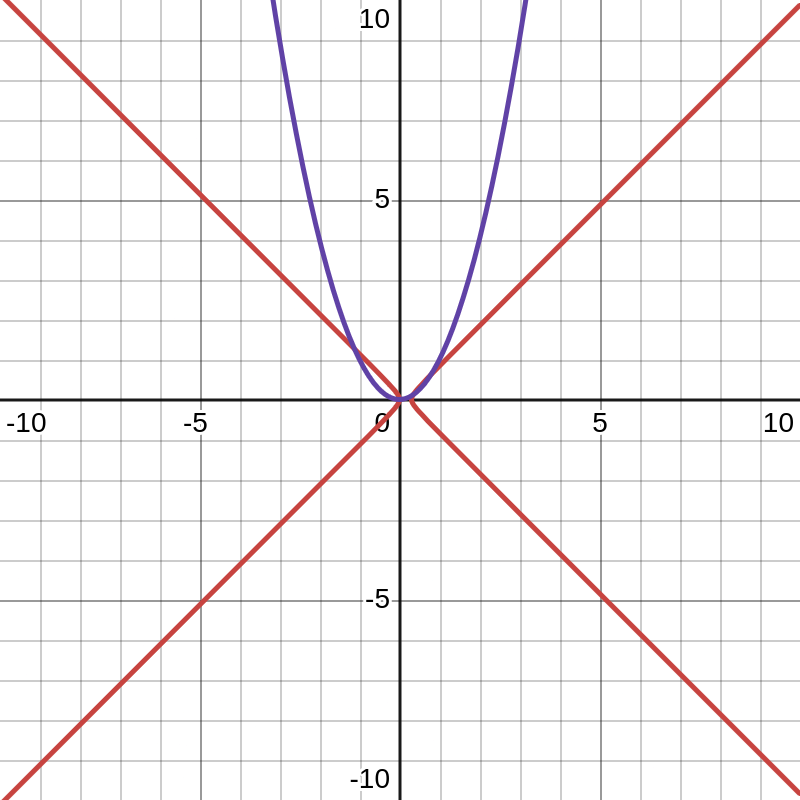
\includegraphics[width=\linewidth]{conic_pic_2.png}

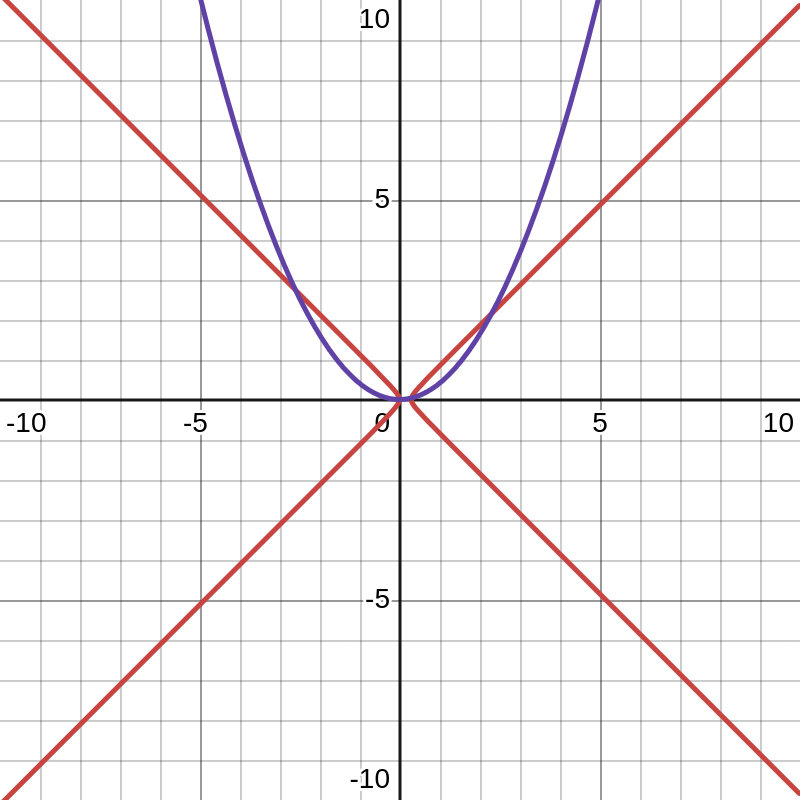
\includegraphics[width=\linewidth]{conic_pic_3.png}


\textbf{359.2}:

Let's denote $m$ as the man, $w$ as the wolf, $g$ as the goat, and $c$ for the cabbage.

We start with $m = w = g = c = 0$ and we want to end up with $m = w = g = c = 1$.

$g \neq c$ when $m \neq g$.
$w \neq g$ when $m \neq g$.

Step 1:

Move the goat to the right bank.

$m = g = 1$ and $w = c = 0$.

Step 2:

Return the man alone.

$g = 1$ and $m = w = c = 0$.

Step 3:

Take the wolf to the right bank.

$m = g = w = 1$ and $c = 0$.

Step 4:

Bring the goat back to the left bank.

$m = g = c = 0$ and $w = 1$.

Step 5:

Move the cabbage to the right bank.

$g = 0$ and $m = w = c = 1$.

Step 6:

Return the man alone.

$m = g = 0$ and $w = c = 1$.

Step 7:

Bring the goat to the right bank.

$m = w = g = c = 1$.


\textbf{359.31}:

The Fibonacci sequence (the sequence of rabbit pairs) is
determined by the recursive rule $F_0 = F_1 = 1$ and $F_n = F_{n-1} + F_{n-2}$.
Show that
\[F_{n+1} \cdot F_{n-1} = F_{n}^2 - (-1)^n\]
and that
\[\lim_{n \to \infty} \frac{F_{n}}{F_{n-1}} = \frac{1 + \sqrt{5}}{2}\]

We will show the first identity $F_{n+1} \cdot F_{n-1} = F_{n}^2 - (-1)^n$
using mathematic induction.

Base case:

For $n=1$:
\[F_2 \cdot F_0 = F_1^2 - (-1)^1\]
\[2 \cdot 1 = 1^2 + 1\]
\[2 = 2\]

The base case holds.

The inductive case:

Assume $F_{k+1} \cdot F_{k-1} = F_{k}^2 - (-1)^k$ for some $k \in \ZZ$.

Using the reursive definition:
\[F_{k+2} = F_{k+1} + F_{k}\]
\[F_{k+1} \cdot F_{k} = (F_{k+1} + F_{k}) \cdot F_k - (-1)^{k+1}\]
\[F_{k+1} \cdot F_k = F_{k+1}^2 + F_k \cdot F_{k+1} - (-1)^{k+1}\]
\[F_{k+1} \cdot F_k = F_{k+1}^2 + F_{k+1} \cdot F_k - (-1)^{k+1}\]

Simplifying gives:
\[F_{k+1}^2 - (-1)^{k+1} = F_{k+1} \cdot F_k\]

Which completes the proof.


For the second identity $\lim_{n \to \infty} \frac{F_n}{F_{n-1}} = \frac{1 + \sqrt{5}}{2}$,
consider the ratio $L = \lim_{n \to \infty} \frac{F_n}{F_{n-1}}$.

We know that $F_n = F_{n-1} + F_{n-2}$. So,
\[\lim_{n \to \infty} \frac{F_n}{F_{n-1}} = \lim_{n \to \infty} \frac{F_{n-1} + F_{n-1}}{F_{n-1}}\]

This can be simplified to $L = 1 + \frac{1}{L}$. Solving for $L$ gives:
\[L^2 = L + 1\]
\[L^2 - L - 1 = 0\]

Applying the quadratic formula gives:
\[L = \frac{1 \pm \sqrt{5}}{2}\]

Since the ratio $L$ must be positive since all Fibonacci numbers are positive,
this becomes $\frac{1 + \sqrt{5}}{2}$.


\textbf{359.40}:

From Oresme's Tractatus de configurationibus qualitatum et motuum:
Show geometrically that the sum of the series
\[48 \cdot 1 + 48 \cdot \frac{1}{4} \cdot 2 + 48 \left(\frac{1}{4}\right)^2 \cdot 4 + \dots + 48 \left(\frac{1}{4}\right)^n \cdot 2^n + \dots\]
is equal to 96.

Each term of the series can be viewed as a rectangle with height
$48 \left(\frac{1}{4}\right)^n$ and width $2^n$.

The rectangle's height quarters every step while its width doubles.
This means each successive rectangle's area halves.

Arranging these rectangles side by side makes them resemble a right triangle.

we can rearrange the rectangles so that it is a shape with height $48$
(that of the first rectangle) and whose width is the limit of
$1 + \frac{1}{2} + \frac{1}{4} + \dots$, which is $2$.

So, the area would be $48 \cdot 2 = 96$.


\textbf{418.33}:

Solve $x^3 + 21x = 9x^2 + 5$ completely by first using the substitution $x = y+3$
to eliminate the term in $x^2$ and then solve the resulting equation in $y$.

Substituting in $x = y + 3$ and doing simplication to eliminate the $y^2$ term gives:
\[y^3 - 6y + 4 = 0\]

Using the cubic equation gives solutions for $y$ as $2$, $-1 + \sqrt{3}$, and $-1 - \sqrt{3}$.
Plugging this back into $x = y + 3$ gives:
\[x = 5\]
\[x = 2 + \sqrt{3}\]
\[x = 2 - \sqrt{3}\]

Plugging these back into the original equation verifies that they are valid solutions.


\end{document}
